% Chapter Template

\chapter{Capture et analyse des besoins} % Main chapter title

\label{Chapter1} % Change X to a consecutive number; for referencing this chapter elsewhere, use \ref{ChapterX}

\lhead{Chapitre 1. \emph{Capture et analyse des besoins}} % Change X to a consecutive number; this is for the header on each page - perhaps a shortened title

%----------------------------------------------------------------------------------------
%	SECTION 1
%----------------------------------------------------------------------------------------

\section{Planning prévisionnel du projet}
\begin{figure}[htbp]
	\centering
		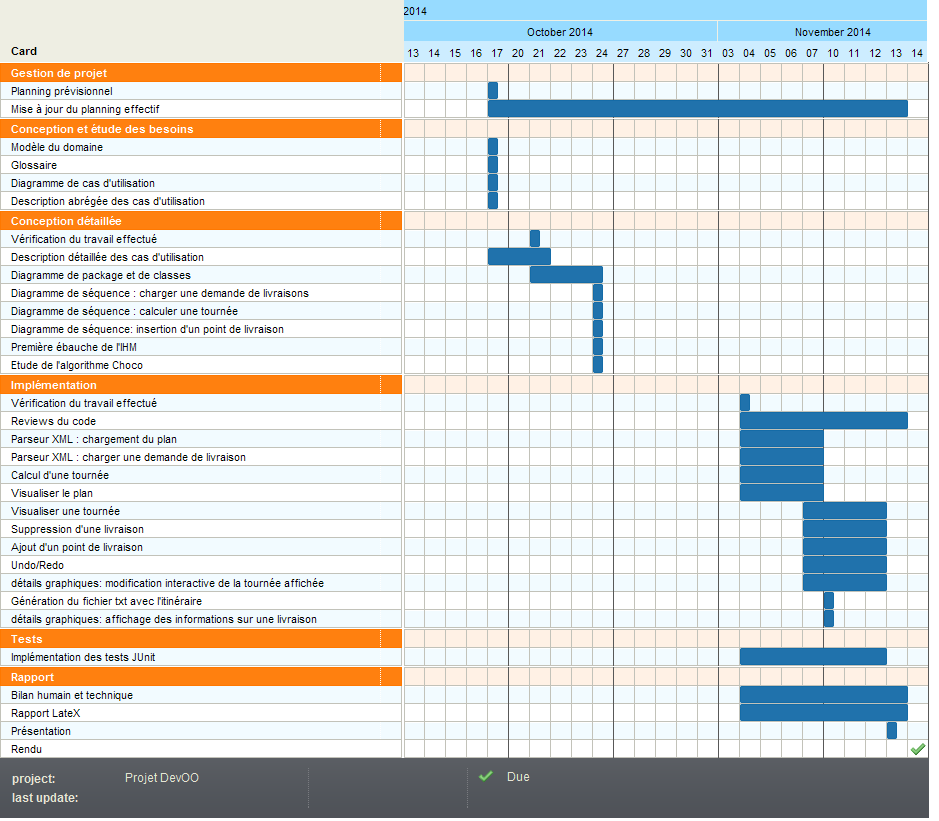
\includegraphics[width=\textwidth,height=\textheight,keepaspectratio]{Figures/previsional_plan}
		\rule{35em}{0.5pt}
	\caption[Planning prévisionnel]{Planning prévisionnel du projet}
\end{figure}

%----------------------------------------------------------------------------------------
%	SECTION 2
%----------------------------------------------------------------------------------------

\section{Modèle du domaine}

\begin{figure}[H]
	\centering
		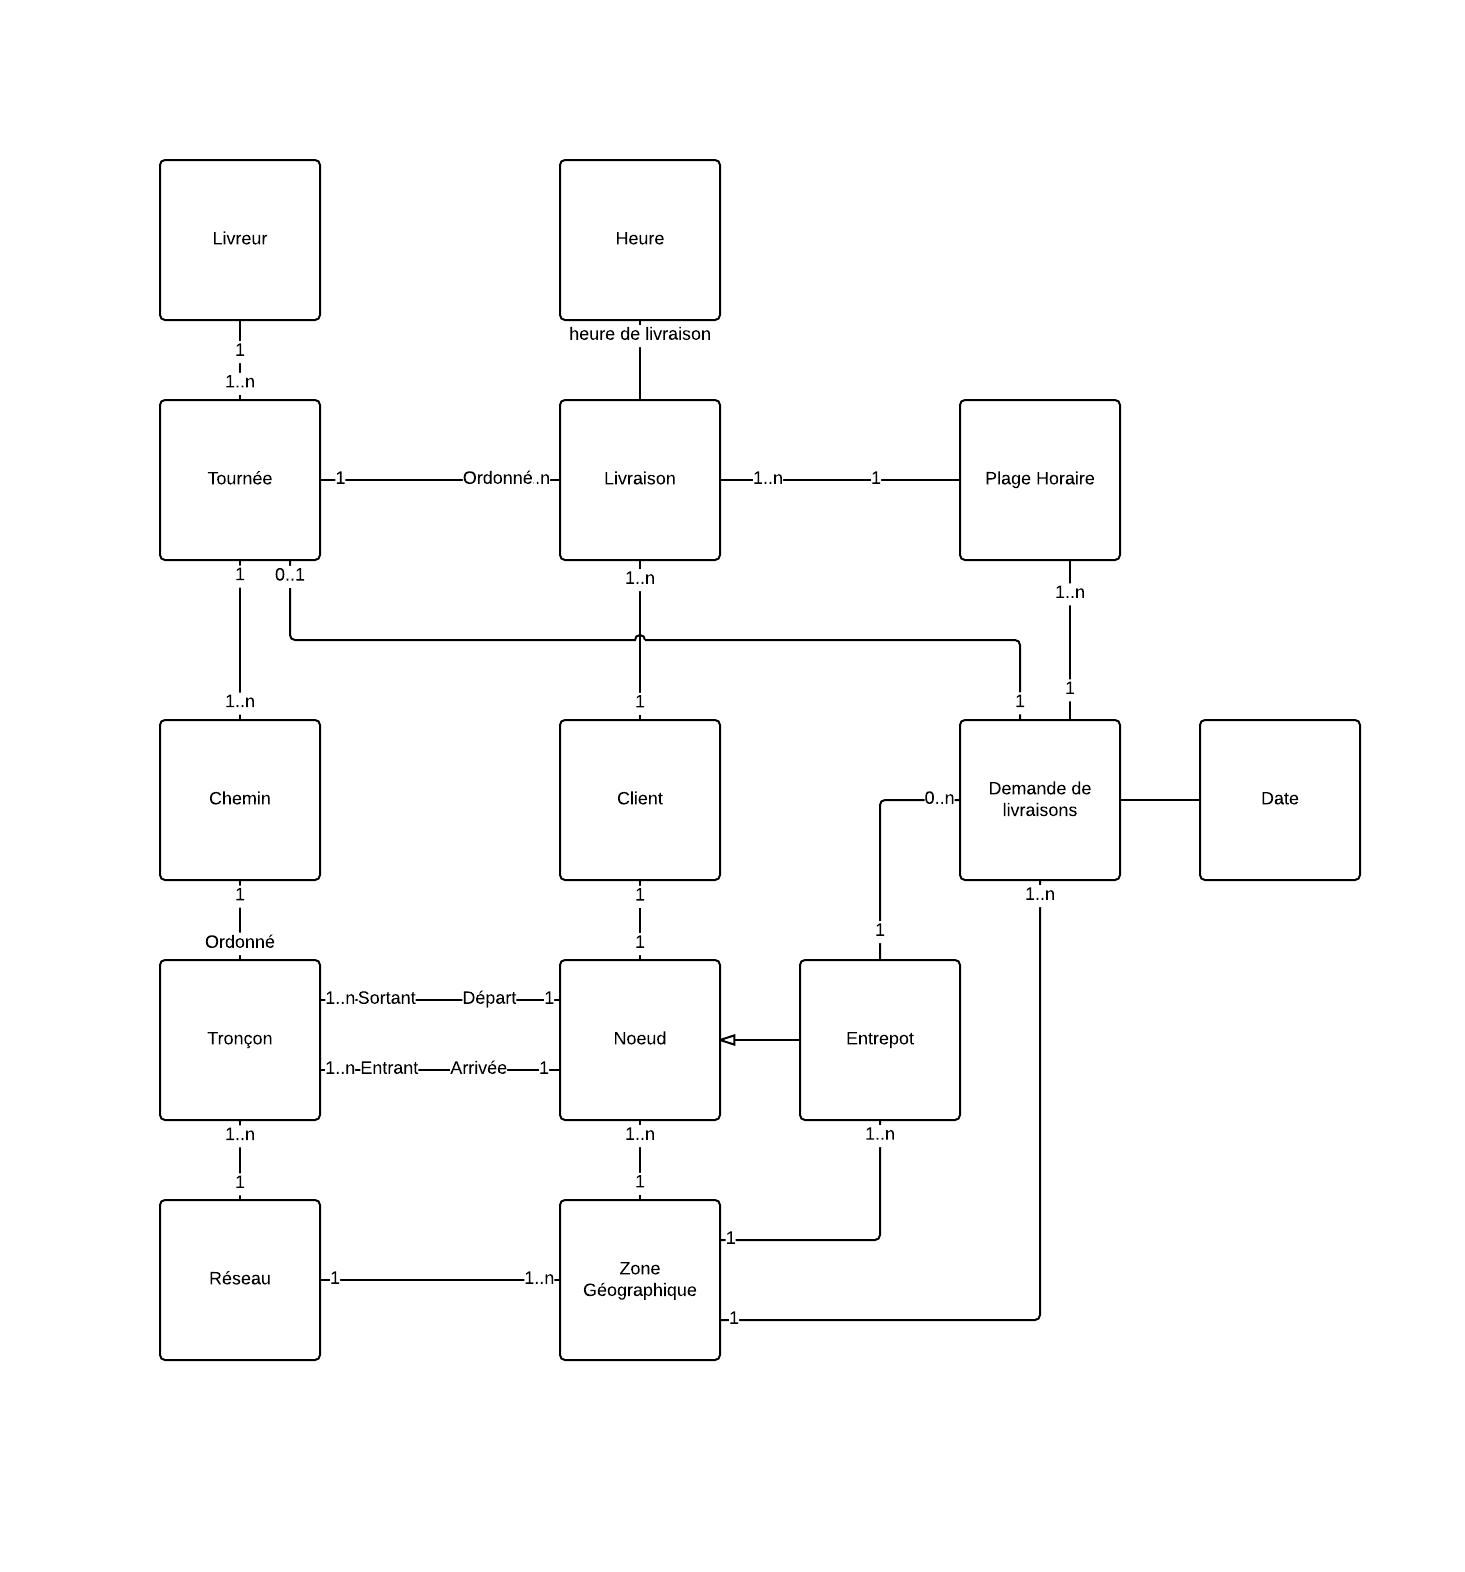
\includegraphics[width=\textwidth,height=\textheight,keepaspectratio]{Figures/modele_domaine}
		\rule{35em}{0.5pt}
	\caption[Modèle du domaine]{Modèle du domaine}
\end{figure}
\clearpage

\section{Diagramme des cas d'utilisations}
\begin{figure}[htbp]
	\centering
		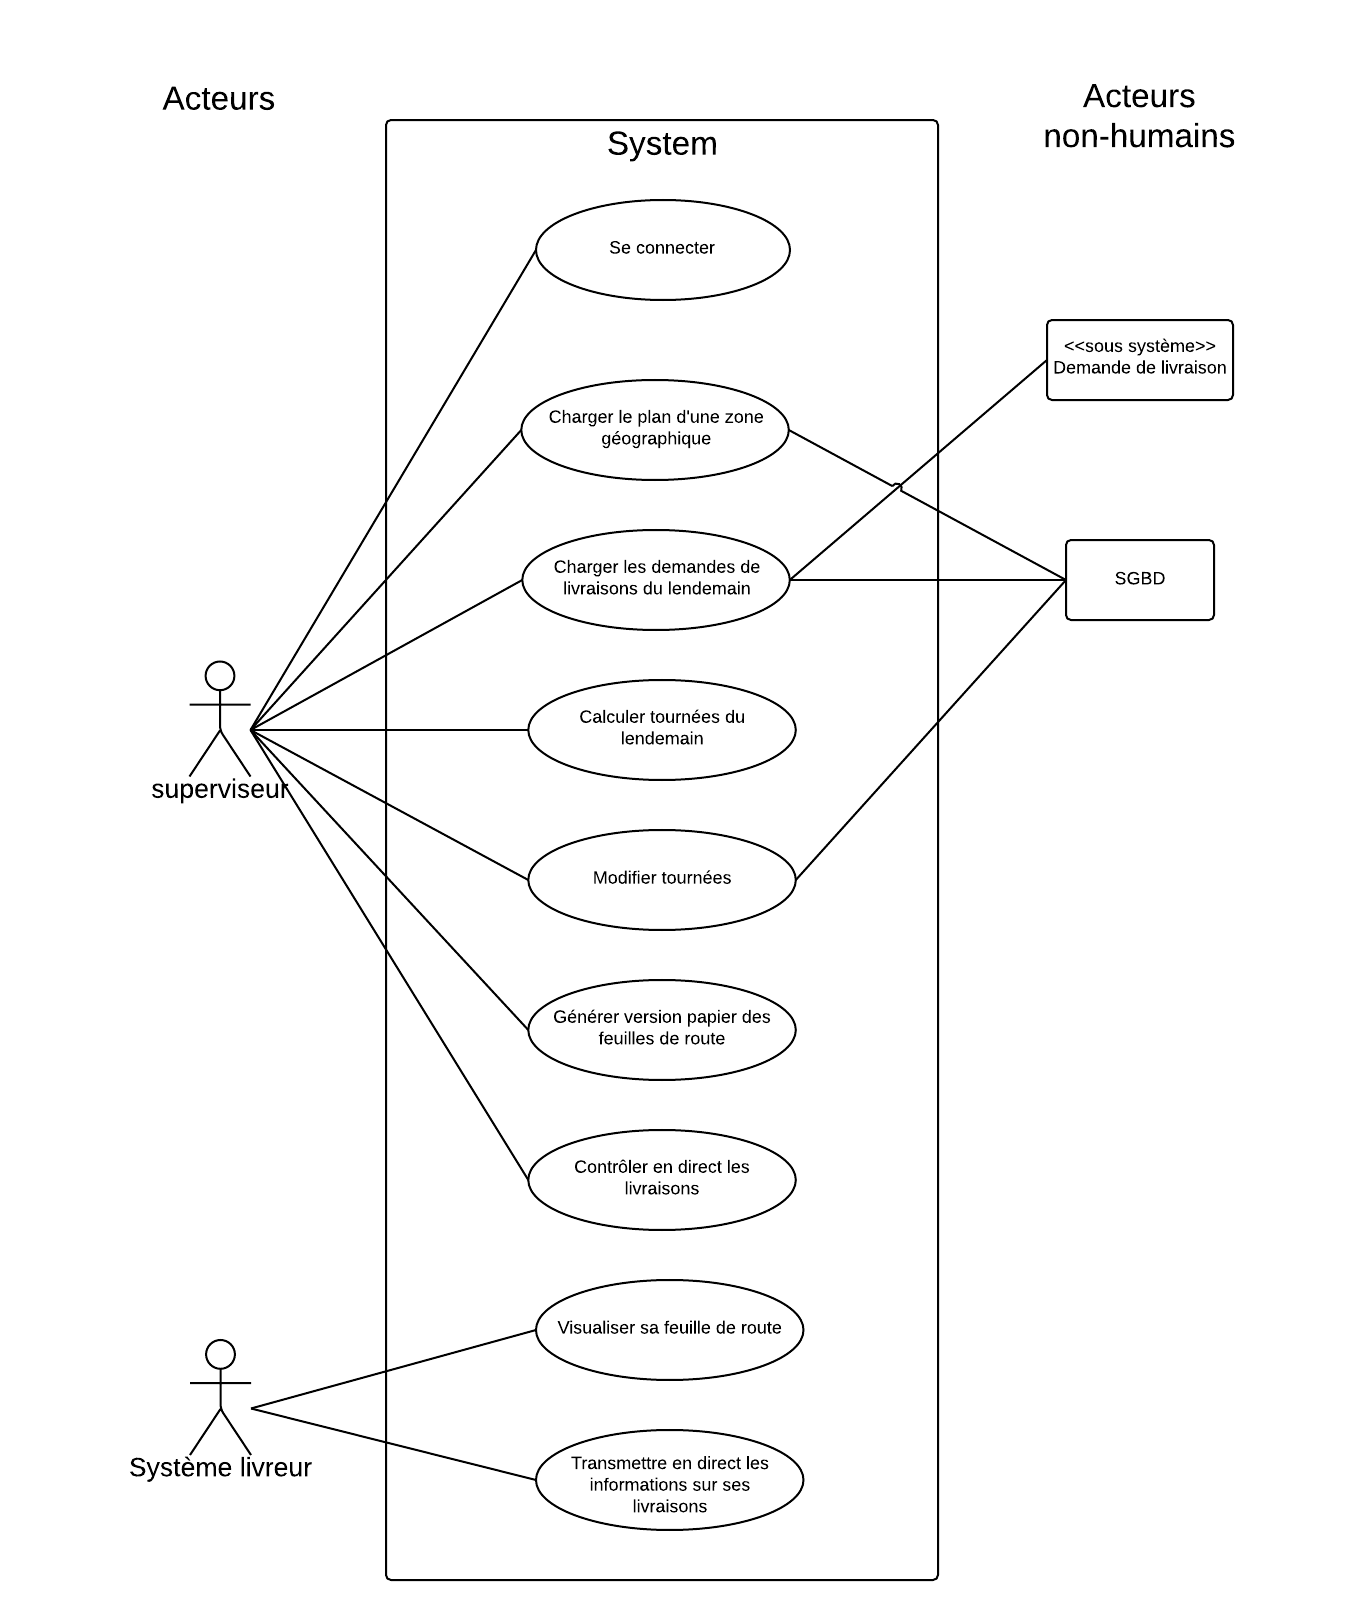
\includegraphics[width=\textwidth,height=\textheight,keepaspectratio]{Figures/cu}
		\rule{35em}{0.5pt}
	\caption[Diagramme des cas d'utilisations]{Diagramme de cas d'utilisations}
\end{figure}
\section{Description textuelle abrégée des cas d'utilisation}
\subsection{Superviseur}
\begin{description}
\item [Se connecter au Système]Le Superviseur rentre son identifiant et son mot de passe pour se connecter.
\item [Charger le plan d’une zone géographique]Le Superviseur fournit au Système le plan de la zone géographique voulue. Le Système valide la saisie du plan.
\item [Charger les demandes de livraison du lendemain]Le sous-système “Demande de livraison” fournit au Système les demandes de livraison du lendemain. Le Système valide la bonne réception et la cohérence des données. 
\item [Calculer les tournées du lendemain]En se basant sur la plan de la zone et les demandes de livraison, le Système calcule les tournées du lendemain. Le Système affiche les tournées au Superviseur et les éventuels problèmes (plages horaires non respectées).
\item [Modifier tournées (avant validation)]Le Superviseur résout les éventuels problèmes en contactant les clients concernés et en modifiant manuellement les tournées en plaçant considérant le ou les nouveaux points et en supprimant l’ancien qui posait problème. Cette suppression entraînant une cassure entre deux points, le Système calcule le plus court chemin entre ces deux points.
\item [Générer version papier des feuilles de route] Le Superviseur valide les tournées puis imprime les feuilles de route (version papier).
\item [Contrôler les livraisons en direct] Le Superviseur consulte le Système pour obtenir les informations sur les livraisons effectuées ou non-effectuées. Ces informations proviennent du Système Livreur qui renvoie les données des livraisons en cours.
Le Superviseur peut modifier interactivement les tournées.
\end{description}
\subsection{Système livreur}
\begin{description}
\item [Visualiser sa feuille de route]Le Système Livreur consulte en direct sa tournée, mise à jour en temps réel avec le Système, car le Superviseur peut la modifier en direct.
\item [Transmettre en direct les informations sur les livraisons]A chaque livraison le Système Livreur envoie un message de confirmation au Système. Si la livraison n’a pas pu être effectuée, le Système Livreur envoie tout de même un message au Système pour signaler son échec.


\end{description}